\documentclass{beamer}
%\documentclass[handout]{beamer}
\mode<presentation>
{
%  \usetheme{Darmstadt}%default Warsaw
  \setbeamercovered{transparent}
}

\setbeamertemplate{navigation symbols}{} 
\newtheorem{thm}{Theorem}[section]
%\useinnertheme[shadow=true]{rounded}

\setbeamercolor{block title}{use=structure,fg=structure.fg,bg=structure.fg!20!bg}
\setbeamercolor{block body}{parent=normal text,use=block title,bg=block title.bg!50!bg}

\usepackage{beamerthemesplit}
\usepackage{epsfig,graphics}
\usepackage{amsmath,amsfonts,amssymb,color,array,subfigure,rotating,texdraw} 
\usepackage{multimedia}
\usepackage{psfrag}
%\usepackage[dvips]{color}
\usepackage[english]{babel}
\usepackage[font=tiny]{caption}

\newcommand{\bDiamond}{\mathbin{\Diamond}}
\newcommand{\bLozenge}{\mathbin{\blacklozenge}}

\makeatletter
\newcommand\bigDiamond{\mathop{\mathpalette\bigDi@mond\relax}}
\newcommand\bigDi@mond[2]{%
  \vcenter{\hbox{\m@th
    \scalebox{\ifx#1\displaystyle 2\else1.2\fi}{$#1\Diamond$}%
  }}%
}
\newcommand\bigLozenge{\mathop{\mathpalette\bigL@zenge\relax}}
\newcommand\bigL@zenge[2]{%
  \vcenter{\hbox{\m@th
    \scalebox{\ifx#1\displaystyle 2\else1.2\fi}{$#1\blacklozenge$}%
  }}%
}
\makeatother


\definecolor{greenn}{rgb}{0.1,0.4,0.1}

\def\Dpartial#1#2{ {\partial #1 \over \partial #2} }
\def\Dpartialmix#1#2#3{ {\partial^2 #1 \over \partial #2\,\partial #3} }
\def\Dpartialn#1#2#3{ {\partial^{#3} #1 \over \partial #2^{#3}} }
\def\Txtint{ {\textstyle\int} }
\def\Txtiint{ {\textstyle\iint} }
\def\Bmp#1{ \begin{minipage}{#1} }
\def\Emp{ \end{minipage} }
\def\Bmpc#1{ \begin{minipage}[c]{#1} }
\def\Bmpt#1{ \begin{minipage}[t]{#1} }
\def\Bmpb#1{ \begin{minipage}[b]{#1} }
\newcommand{\stitle}[1]{\centering{{\sc \Large #1 }}\vskip .5cm}
\def\H{{\mathcal{H}}}
\def\J{{\mathcal{J}}}
\def\hdo{\dot{H}^1}
\def\pat{\Phi_{\alpha,T}}
\def\ppat{\Phi'_{\alpha,T}}

\def\A{{\mathcal{A}}}
\def\B{{\mathcal{B}}}
\def\E{{\mathcal{E}}}
\def\K{{\mathcal{K}}}
\def\L{{\mathcal{L}}}
\def\M{{\mathcal{M}}}
\def\O{{\mathcal{O}}}
\def\F{{\mathcal{F}}}
\def\N{{\mathcal{N}}}
\def\T{{\mathcal{T}}}
\def\P{{\mathcal{P}}}
\def\R{{\mathcal{R}}}
\def\K{{\mathcal{K}}}
\def\C{{\mathcal{C}}}
\def\U{{\mathcal{U}}}
\def\S{{\mathcal{S}}}
\def\DD{{\mathcal{D}}}
\def\QQ{{\mathcal{Q}}}
\def\NS{{\mathcal{NS}}}
\def\l{{\ell}}


\newcommand{\bds}{\boldsymbol}
\newcommand{\la}{\left\langle}
\newcommand{\ra}{\right\rangle}
\newcommand{\lb}{\left\lbrace}
\newcommand{\rb}{\right\rbrace}

\def\BB{{\mathbb{B}}}
\def\KK{{\mathbb{K}}}
\def\RR{{\mathbb{R}}}
\def\TT{{\mathbb{T}}}
\def\ZZ{{\mathbb{Z}}}
\def\CC{{\mathbb{C}}}

\def\tu{{\tilde{u}}}
\def\ta{{\tilde{a}}}
\def\tb{{\tilde{b}}}

\def\magenta#1{{\color{magenta}{ #1 }}}
\def\red#1{{\color{red}{ #1 }}}
\def\blue#1{{\color{blue}{ #1 }}}
\def\green#1{{\color{green}{ #1 }}}
\def\white#1{{\color{white}{ #1 }}}
\def\black#1{{\color{black}{ #1 }}}

\def\bC{{\bf C}}
\def\bG{{\bf G}}
\def\bZ{{\bf Z}}

\newcommand{\mbb}[1]{\mathbb{#1}}
\newcommand{\mc}[1]{\mathcal{#1}}

\def\a{\hat{\text{a}}}
\def\P{{\mathcal{P}}}
\def\b{{\bf b}}
\def\bn{{\boldsymbol \nabla}}
\def\be{{\boldsymbol \eta}}
\def\bep{{\boldsymbol \eta'}}
\def\bea{{\boldsymbol \eta_\alpha}}
\def\bena{{\boldsymbol \eta_\alpha^{(n)}}}
\def\beza{{\boldsymbol \eta_\alpha^0}}
\def\benpa{{\boldsymbol \eta_\alpha^{(n+1)}}}
\def\bepa{{\boldsymbol \eta'_\alpha}}
\def\upa{\boldsymbol u'_\alpha}
\def\usa{\boldsymbol u^*_\alpha}
\def\f{{\bf f}}
\def\q{{\bf q}}
\def\r{{\bf r}}
\def\d{{\bf d}}
\def\v{{\bf v}}
\def\z{{\bf z}}
\def\y{{\bf y}}
\def\k{{\bf k}}
\def\x{{\bf x}}
\def\m{{\bf m}}
\def\l{{\bf l}}
\def\n{{\bf n}}
\def\e{{\bf e}}
\def\j{{\bf j}}
\def\D{{\bf D}}
\def\X{{\bf X}}
\def\Q{{\bf Q}}
\def\g{{\bf G}}
\def\w{{\bf w}}
\def\u{{\bf u}}
\def\ua{\boldsymbol u_\alpha}
\def\f{{\bf f}}
\def\y{{\bf y}}
\def\0{{\mathbf{0}}}
\def\V{{\mathbf{V}}}
\def\W{{\mathbf{W}}}
\def\Z{{\mathbf{Z}}}


\def\tT{{\tilde{\mathcal{T}}}}
\def\tZ{{\tilde{\mathcal{Z}}}}

\newcommand{\tuE}{\widetilde{\mathbf{u}}_{\E_0}}
\newcommand{\tuET}{\widetilde{\u}_{0;\E_0,T}}
\newcommand{\uET}{\u_{0;\E_0,T}}
\newcommand{\ET}{\E_T(\u_0)}
\def\tTE{\widetilde{T}_{\E_0}}

\def\btau{{\bf \tau}}
\def\hu{{\hat{u}}}
\def\bnabla{\boldsymbol{\nabla}}
\def\bphi{\boldsymbol{\phi}}
\def\bDelta{\boldsymbol{\Delta}}
\def\bPhi{\boldsymbol{\Phi}}
\def\bxi{\boldsymbol{\xi}}
\def\etab{\boldsymbol{\eta}}
\def\control{{\phi}}
\def\controlpert{{\phi'}}
\def\bsigma{\boldsymbol{\sigma}}
\def\bomega{\boldsymbol{\omega}}
\def\teta{\widetilde{\boldsymbol{\eta}}}

\newcommand{\argmin}{\operatorname{argmin}}
%\newcommand{\argmax}{\operatorname{argmax}}
\DeclareMathOperator*{\argmax}{argmax}
\newcommand{\sgn}{\operatorname{sgn}}
\newcommand{\sign}{\operatorname{sign}}
\newcommand{\rank}{\operatorname{rank}}
\newcommand{\Ext}{\operatorname{Ext}}
\newcommand{\id}{\,\mathrm{d}}
\newcommand{\Id}{\operatorname{Id}}
\newcommand{\Ker}{\operatorname{Ker}}
\newcommand{\kvec}{\mathbf{k}}

\newcommand{\sigdis}{\sigma_{\text{disc}}}
\newcommand{\sigess}{\sigma_{\text{ess}}}
\def\sigp{\sigma_{\text{p}}}
\def\mumax{\mu_{\text{max}}}

\long\def\symbolfootnote[#1]#2{\begingroup%
\def\thefootnote{\fnsymbol{footnote}}\footnote[#1]{#2}\endgroup} 

%%%%%%%%%%%%%%%%%%%%%%%%%%%%%%%%%%%%%%%%%%%%%%%%%%%%%%%%%%%%%%%%%%%%%%%%%%
%%%%%%%%%%%%%%%%%%%%%%%%%%%%%%%%%%%%%%%%%%%%%%%%%%%%%%%%%%%%%%%%%%%%%%%%%%
%%%%%%%%%%%%%%%%%%%%%%%%%%%%%%%%%%%%%%%%%%%%%%%%%%%%%%%%%%%%%%%%%%%%%%%%%%

\title{Systematic Search for Singularities in 3D Euler-Voigt Flows}
\author[\underline{N. Bensler}, B.~Protas, and X.~Zhao]{\underline{Noah Bensler}$^{1}$, Bartosz Protas$^{1}$, Xinyu Zhao$^{1,2}$}
\institute{
$^{1}$Department of Mathematics \& Statistics \\
McMaster University, Hamilton, Ontario, Canada \\ \vspace*{0.3cm}
$^2$Department of Mathematical Sciences, New Jersey Institute of Technology, \\
Newark, NJ 07103, USA \\ \vspace*{0.3cm}
%\footnotesize
Funded by NSERC (Canada), Computing Time Provided by {\sc Compute Canada} \vspace*{-0.25cm} }
%\vspace*{-0.2cm}

\date{\medskip
March 9, 2026  \\ \smallskip}


\begin{document}

\frame{\titlepage}


%\section[Agenda]{}
\frame{
\frametitle{Agenda}
\tableofcontents
}

%%%%%%%%%%%%%%%%%%%%%%%%%%%%%%%%%%%%%%%%%%%%%%%%%%%%%%%%%%%%%%%%%%%%%%%%%%
%%%%%%%%%%%%%%%%%%%%%%%%%%%%%%%%%%%%%%%%%%%%%%%%%%%%%%%%%%%%%%%%%%%%%%%%%%
%%%%%%%%%%%%%%%%%%%%%%%%%%%%%%%%%%%%%%%%%%%%%%%%%%%%%%%%%%%%%%%%%%%%%%%%%%
\section{Introduction}
\frame{
\centering

\LARGE
{Singularities \& Euler-Voigt Flows}
}

\subsection{Singularities \& Euler-Voigt Flows}

\frame
{
\hspace*{-1.0cm}
\Bmp{12cm}
\raggedright

\begin{itemize}
\item<1->
Navier-Stokes system ($\Omega = [0,L]^3$)
%\footnotesize
\small
\begin{equation*}
\left\{
\begin{aligned}
&\partial_{t}\u+({\u}\cdot{\bnabla}){\u}
+{\bnabla}{p}-\nu\Delta{{\u}}=\0,  && \text{in} \ \Omega\times(0,T] \\ 
&{\bnabla}\cdot{\u}=0,                     && \text{in} \ \Omega\times(0,T] \\ 
&\u = \be                &&  \text{in} \ \Omega \ \text{at} \ t=0 \\
&\textrm{Periodic Boundary Conditions}                  &&  \text{on} \ \partial\Omega\times(0,T] 
\end{aligned}
%\label{eq:NS}
\right.
\end{equation*}
\medskip

\item<2->
{\bf The Big Question:} \\ \smallskip
{\blue{\em   Given a smooth initial condition $\be$, does the Navier-Stokes system always admit smooth solutions $\u(t)$ for arbitrarily long times $t$? }} \\ \smallskip

\bigskip

\item<3->
One of the Clay Institute ``Millennium Problems'' (\$ 1M prize!) \\
\smallskip
\scriptsize
\qquad
{\tt{https://www.claymath.org/millennium/navier-stokes-equation/}}

\end{itemize}
\Emp
}


\frame
{
\hspace*{-1.0cm}
\Bmp{12cm}
\raggedright

\begin{itemize}
\item<1->
Euler system ($\Omega = [0,L]^3$)
%\footnotesize
\small
\begin{equation*}
\left\{
\begin{aligned}
&\partial_{t}\u+({\u}\cdot{\bnabla}){\u}
+{\bnabla}{p}=\0,  && \text{in} \ \Omega\times(0,T] \\ 
&{\bnabla}\cdot{\u}=0,                     && \text{in} \ \Omega\times(0,T] \\ 
&\u = \be                 &&  \text{in} \ \Omega \ \text{at} \ t=0 \\
&\textrm{Periodic Boundary Conditions}                  &&  \text{on} \ \partial\Omega\times(0,T]
\end{aligned}
%\label{eq:NS}
\right.
\end{equation*}
\medskip

\item<2->
{\bf The Big Question:} \\ \smallskip
{\blue{\em   Given a smooth initial condition $\be$, does the Euler system always admit smooth solutions $\u(t)$ for arbitrarily long times $t$? }} \\ \smallskip

\bigskip

\item<3->
There is numerical evidence for singularity formation in Euler (J.D. Gibbon 2008).

\end{itemize}
\Emp
}

\frame
{
\hspace*{-1.0cm}
\Bmp{12cm}
\raggedright

\begin{itemize}
\item<1->
Euler-Voigt system ($\Omega = [0,L]^3$)
%\footnotesize
\small
\begin{equation*}
\left\{
\begin{aligned}
&\blue{-\alpha^2\partial_{t}\Delta\ua} +\partial_{t}\ua+({\ua}\cdot{\bnabla}){\ua}
+{\bnabla}{p}=\0,  && \text{in} \ \Omega\times(0,T] \\ 
&{\bnabla}\cdot{\ua}=0,                     && \text{in} \ \Omega\times(0,T] \\ 
&\ua = \be_\alpha                 &&  \text{in} \ \Omega \ \text{at} \ t=0 \\
&\textrm{Periodic Boundary Conditions}                  &&  \text{on} \ \partial\Omega\times(0,T]
\end{aligned}
%\label{eq:NS}
\right.
\end{equation*}
\smallskip

\item<2->
$\alpha > 0$ is the regularization parameter with units of length. Acts as a 'spectral filter'. The Euler-Voigt system is globally well-posed given smooth initial conditions (Y. Cao et al. 2006). 
\medskip

\item<3->
As $\alpha\rightarrow 0$ the solutions of Euler-Voigt converge to the solutions of Euler and so its behaviour can be used to determine if the Euler equations will develop a finite-time singularity.

\end{itemize}
\Emp
}

%%%%%%%%%%%%%%%%%%%%%%%%%%%%%%%%%%%%%%%%%%%%%%%%%%%%%%%%%%%%%%%%%%%%%%%%%%
%%%%%%%%%%%%%%%%%%%%%%%%%%%%%%%%%%%%%%%%%%%%%%%%%%%%%%%%%%%%%%%%%%%%%%%%%%
%%%%%%%%%%%%%%%%%%%%%%%%%%%%%%%%%%%%%%%%%%%%%%%%%%%%%%%%%%%%%%%%%%%%%%%%%%

\subsection{Finite-time Blow-up Criteria}

\frame
{
\hspace*{-1.0cm}
\Bmp{12cm}
\raggedright

\begin{itemize}
\item<1-> Proven by Theorem 1 in (A. Larios et al. 2018).
\begin{thm}\label{thm:Theorem:1.1}
Let $\bea\in H^s$, $s\geq 3$ with $\bn \cdot \bea = 0$ and let $\ua$ be the corresponding unique solution of Euler-Voigt. Suppose that there exists a time $T^*>0$ such that
\begin{equation}
\limsup_{\alpha \rightarrow 0^+} \left( \alpha \sup_{t\in[0,T^*]} \|\bn \ua(t)\|_{L^2}\right) > 0.
\end{equation}
Then the Euler equations with the initial condition $\be_\alpha$ must develop a singularity within the interval $[0,T^*]$.
\end{thm}

\end{itemize}
\Emp
}

\frame
{
\hspace*{-1.0cm}
\Bmp{12cm}
\raggedright

\begin{itemize}
\item<1-> Theorem 5.1 (A. Larios et al. 2010).
\begin{thm}\label{thm:Theorem:1.2}
Given initial data $\be,\bea \in H^s(\TT^3)$ for some $s\geq 3$, let
$$\u,\ua \in C([0,T],H^s(\TT^3)) \cap C^1([0,T],H^{s-1}(\TT^3))$$
be the corresponding solutions to Euler and Euler-Voigt, respectively, where $0<T<T_{\text{max}}$ and $T_{\text{max}}$ is the maximal time for which a solution to Euler exists and is unique. For all $t\in[0,T]$, we have 
\begin{subequations}
\begin{align*}
&\|\u(t)-\ua(t)\|_{L^2}^2 + \alpha^2\|\bn(\u(t)-\ua(t))\|_{L^2}^2 \leq \\ 
&\left( \|\be-\bea \|_{L^2}^2 + \alpha^2\|\bn(\be - \bea)\|_{L^2}^2 \right)e^{Ct} + C\alpha^2(e^{Ct}-1).
\end{align*}
\end{subequations}
\end{thm}

\end{itemize}
\Emp
}

\frame
{
\hspace*{-1.0cm}
\Bmp{12cm}
\raggedright

\begin{itemize}
\item<1-> Modified from Theorem 5.2 (A. Larios et al. 2010).
\begin{thm}\label{thm:Theorem:1.3}
Given initial data $\be,\bea \in H^s(\Omega)$ for some $s\geq 3$ satisfying
\begin{equation*}
\|\be-\bea\|_{L^2}^2+\alpha^2\|\bnabla(\be-\bea)\|_{L^2}^2 \rightarrow 0, \quad \text{as } \alpha\rightarrow 0,
\end{equation*} 
let $\u,\ua \in C([0,T],H^s(\Omega))\cap C^1([0,T],H^{s-1}(\Omega))$ be the corresponding solutions to Euler and Euler-Voigt, respectively. If there exists a finite time $T^*>0$ such that the solutions $\ua$ satisfies
\begin{equation*}
\limsup_{\alpha \rightarrow 0} \left( \alpha^2 \sup_{t\in[0,T^*]} \|\bnabla \ua(t)\|_{L^2}^2\right) > 0,
\end{equation*}
then $\u$ develops a singularity in the interval $[0,T^*]$.
\end{thm}


\end{itemize}
\Emp
}

\frame
{
\hspace*{-1.0cm}
\Bmp{12cm}
\raggedright

\begin{proof}\renewcommand{\qedsymbol}{}
Suppose that the solution $\u$ of the Euler equations Euler with the initial condition $\be$ is regular on $[0,T^*]$. Since the Euler-Voigt equations are globally well-posed, we have
\begin{equation*}
\|\ua(t)\|_{L^2}^2 + \alpha^2\|\bn\ua(t)\|_{L^2}^2  = \|\bea\|_{L^2}^2+\alpha^2\|\bn\bea\|_{L^2}^2,
\end{equation*}
thus
\begin{equation*}
\alpha^2\|\bn\ua(t)\|_{L^2}^2  = \|\bea\|_{L^2}^2+\alpha^2\|\bn\bea\|_{L^2}^2 - \|\ua(t)\|_{L^2}^2.
\end{equation*}
Taking the supremum over $t\in[0,T^*]$ of the above equation, we obtain that
\begin{equation*}
\sup_{t\in[0,T^*]}\alpha^2\|\bn\ua(t)\|_{L^2}^2  = \|\bea\|_{L^2}^2+\alpha^2\|\bn(\bea)\|_{L^2}^2 - \inf_{t\in[0,T^*]} \|\ua(t)\|_{L^2}^2.
\end{equation*}
\end{proof}

\Emp
}

\frame
{
\hspace*{-1.0cm}
\Bmp{12cm}
\raggedright

\begin{proof}[\proofname\ (Cont.)]\renewcommand{\qedsymbol}{}
Taking the limsup as $\alpha\rightarrow 0$, we obtain that
\begin{scriptsize}
\begin{subequations}
\begin{align*}
\limsup_{\alpha\rightarrow 0}\left(\sup_{t\in[0,T^*]}\!\alpha^2\|\bn\ua(t)\|_{L^2}^2\right) &= \limsup_{\alpha\rightarrow 0}\left(\|\bea\|_{L^2}^2+\alpha^2\|\bn(\bea)\|_{L^2}^2 - \!\!\!\inf_{t\in[0,T^*]} \|\ua(t)\|_{L^2}^2\right) \\
&= \|\be\|_{L^2}^2 - \|be\|_{L^2}^2 \\
&= 0
\end{align*}
\end{subequations}
\end{scriptsize}
which contradicts the hypothesis in the theorem that the above expression is positive.
\end{proof}

\Emp
}

\frame
{
\hspace*{-1.0cm}
\Bmp{12cm}
\raggedright

\begin{proof}[\proofname\ (Cont.)]
The second equality holds because
\begin{small}
\begin{subequations}
\begin{align*}
\limsup_{\alpha\rightarrow 0}\left| \inf_{t\in[0,T^*]} \|\ua(t)\|_{L^2} - \|\be\|_{L^2} \right| &\leq \limsup_{\alpha\rightarrow 0}\|\ua(t_\alpha) - \be\|_{L^2}^2 \\
&\leq \limsup_{\alpha\rightarrow 0}\|\ua(t_\alpha) - \u(t_\alpha)\|_{L^2}^2 + \|\u(t_\alpha) - \be\|_{L^2}^2 \\
&= 0.
\end{align*}
\end{subequations}
\end{small}

Here we use the fact that the convergence of the solutions of the Euler-Voigt equations to the solution of the Euler equations is uniform on $[0,T^*]$, as shown in Theorem 5.1.
\end{proof}


\Emp
}

\subsection{Initial Conditions}

\frame
{
\hspace*{-1.0cm}
\Bmp{12cm}
\raggedright

\begin{itemize}
\item<1->
We consider analytic initial conditions that belong to the following Gevrey class
\small
\begin{equation*}\label{eq:Gevrey:Class}
G^\sigma := \lb \v\in H^s(\Omega) : \|\v\|_{G^\sigma} = \la \v,\v\ra_{G^\sigma}^{1/2}<\infty \rb, \quad s\geq 3, \quad \sigma > 0.
\end{equation*}

\item<2->
We select the following inner product
\begin{subequations}\label{eq:Gevrey:Inner:Product}
\begin{align*}
\forall \v,\u \in G^\sigma, \quad \la \v,\u \ra_{G^\sigma} :=& \sum_{\j\in \ZZ^3} (1+|2\pi \j|^2)^se^{4\pi\sigma|\j|}\hat{\v}_{\j}\cdot \overline{\hat{\u}}_{\j} \\
=& \int_{\Omega}(1+|D|^2)^se^{2\sigma |D|}\v\cdot \u \, d\x. \\
=& \la (1+|D|^2)^se^{2\sigma|D|}\v,\u\ra_{L^2}
\end{align*}
\end{subequations}

\item<3->
The operators $|D|$ and $e^{\sigma|D|}$ are defined via
\begin{equation*}\label{eq:D}
\left[ \widehat{|D|\boldsymbol v} \right]_{\boldsymbol j} := 2\pi|\boldsymbol j|\boldsymbol{\hat{v}_j}, \qquad \left[ \widehat{e^{\sigma |D|}\boldsymbol v} \right]_{\boldsymbol j} := e^{2\pi|\boldsymbol j|}\boldsymbol{\hat{v}_j}.
\end{equation*}

\end{itemize}
\Emp
}


\frame
{
\hspace*{-1.0cm}
\Bmp{12cm}
\raggedright

\begin{itemize}
\item<1->
We assume zero mean velocity without loss of generality.

\begin{equation*}
V := \{\boldsymbol v \in G^\sigma : \boldsymbol \nabla \cdot \boldsymbol v = 0, \quad \int_{\Omega}\boldsymbol v\, d\x = 0\}.
\end{equation*}

\item<2->
We use a closed manifold $\M_1 \subset V$ defined as
\begin{equation*}
\M_1 = \{\v \in V : \|\v\|_{\hdo} = \red{C}\}.
\end{equation*}

\item<3->
Euler $(\u)$ and Euler-Voigt $(\ua)$ time scaling property
\begin{equation}
\tilde{\u}_{(\alpha)}(\x,t) = \lambda \u_{(\alpha)}(\x,\lambda t),
\end{equation}

\end{itemize}
\Emp
}

\frame
{
\hspace*{-1.0cm}
\Bmp{12cm}
\raggedright

\begin{itemize}

\item<1->
Taylor Green Vortex $(\Omega = [0,L]^3)$
\begin{equation*}
\be_{TGV} = \begin{bmatrix}
V_0\sin(2\pi x/L)\cos(2\pi y/L)\cos(2\pi z/L) \\
-V_0\cos(2\pi x/L)\sin(2\pi y/L)\cos(2\pi z/L) \\
0
\end{bmatrix}
\end{equation*}

\item<2->
Characteristic time-scale
\begin{equation*}
t_c = \frac{L}{V_0} 
\end{equation*}
\smallskip

\item<3->
Using $(\Omega = [0,2\pi]^3)$ and $V_0 = 1$, Bustamente et a. (2012) showed numerical evidence for finite-time singularity in Euler from $\be_{TGV}$ at $T^* \approx 4$. We use $(\Omega = [0,1]^3)$ and so scale down to $V_0 = 1/2\pi$.  

\end{itemize}
\Emp
}

\frame
{
\hspace*{-1.0cm}
\Bmp{12cm}
\raggedright

\begin{itemize}

\item<1->
Calculate C analytically
\begin{equation*}
\red{C} = \|\be\|_{\hdo} = \|\nabla\be\|_{L^2} = \left[ \sum_{i,j=1}^3 \int_{\Omega} (\partial_i\be_j)^2 \,dx \right]^{1/2}
\end{equation*}

\item<2->
Calculating for scaled $\be_{TGV}$
\begin{equation*}
\|\be_{TGV}\|_{\hdo} = \sqrt{3}/2
\end{equation*}

\item<3->
Create the manifold
\begin{equation*}
\M_1 = \{\v \in V : \|\v\|_{\hdo} = \sqrt{3}/2 \}.
\end{equation*}

\end{itemize}
\Emp
}

\frame
{
\hspace*{-1.0cm}
\Bmp{12cm}
\raggedright

\begin{itemize}

\item<1->
Beale-Kato-Majda (BKM) criterion (Beale et al. 1984): A Smooth solution $u$ of the Euler system develops a singularity at $t=t_0$ if and only if
\begin{equation*}
\lim_{t\rightarrow t_0}\int_0^t \|\omega\|_{L^\infty} d\tau = \infty, \qquad \bds\omega = \nabla \times \u
\end{equation*}

\begin{figure}
\centering
\begin{minipage}[t]{.45\textwidth}
  \centering
  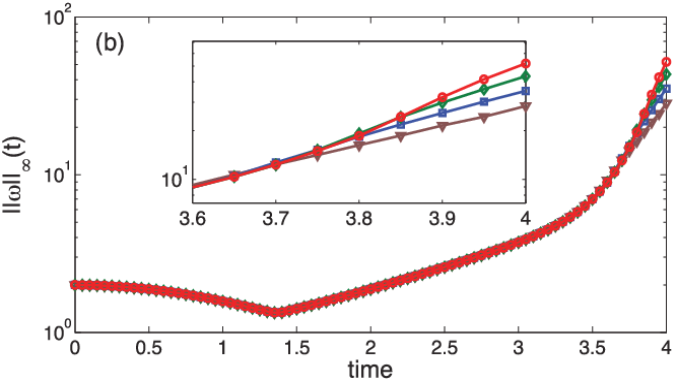
\includegraphics[width=.9\linewidth]{interplay_vorticity_b.png}
  \caption{(Bustamente et al. 2012 Fig. 1b) Maximum of vorticity $\|\omega(\cdot,t)\|_\infty$. Results from runs performed at different resolutions are displayed together: $512^3$ (brown triangles), $1024^3$ (blue squares), $2048^3$ (green diamonds), and $4096^3$ (red circles).}
  
\end{minipage}%
\begin{minipage}[t]{.45\textwidth}
  \centering
  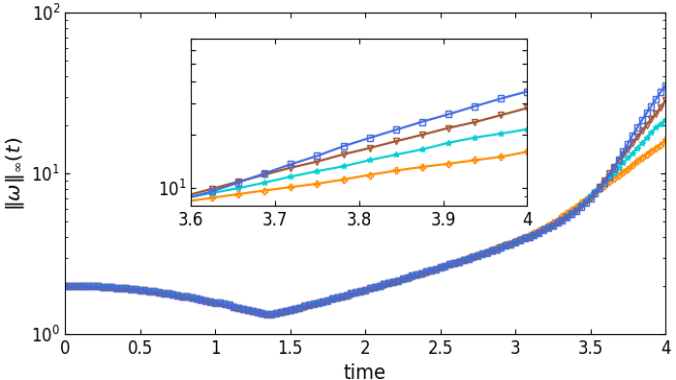
\includegraphics[width=.9\linewidth]{Figure_1.png}
  \caption{Maximum of vorticity $\|\omega(\cdot,t)\|_\infty$. Results from runs performed at different resolutions are displayed together: $128^3$ (orange plus), $256^3$ (cyan star), $512^3$ (brown triangles), $1024^3$ (blue squares).}

  
\end{minipage}
\end{figure}

\end{itemize}
\Emp
}

\section{Optimization Problem for Euler-Voigt}

\frame{
\centering

\LARGE
{Optimization Problem for Euler-Voigt}
}

\subsection{Formulation of the Optimization Problem}
\frame
{
\hspace*{-1.0cm}
\Bmp{12cm}
\raggedright

\begin{itemize}
\item<1->
Define our objective function $\pat : V\rightarrow \RR^+$
\begin{equation*}\label{eq:objective:function}
\pat(\be) := \|\nabla \ua(T;\bea)\|_{L^2}^2 = \|\ua(T;\bea)\|_{\hdo}^2
\end{equation*}
\smallskip

\item<2->
Given $\alpha$,$T \in \RR^+$, find
\begin{equation*}
\tilde{\be}_{\alpha,T} = \argmax_{\bea\in \M_1} \pat(\bea).
\end{equation*}

\item<3->
If $\alpha^2\pat(\tilde{\be}_{\alpha,T})>0$ as $\alpha \rightarrow 0$ then a singularity forms in Euler the interval $[0,T]$.

\end{itemize}
\Emp
}

\subsection{Evaluation of the Gradient}

\frame
{
\hspace*{-1.0cm}
\Bmp{12cm}
\raggedright

\begin{itemize}

\item<1->
The first order finite difference equation for the G$\a$teaux differential $\ppat(\bea;\bepa) : V\times V \rightarrow \RR$,
\begin{equation*}
\ppat(\bea;\bepa):=\lim_{\epsilon\rightarrow 0}\frac{1}{\epsilon}\left[\pat(\bea+\epsilon\bepa)-\pat(\bea)\right].
\end{equation*}

\item<2->
Substituting perturbations into Euler-Voigt
\begin{equation*}
\ua\rightarrow\ua+\upa, \bea\rightarrow\bea+\bepa, \text{ and } p\rightarrow p+p'
\end{equation*}

\item<3->
Linearization of Euler-Voigt
\begin{small}
\begin{subequations}\label{eq:Euler-Voigt:linearization}
\begin{align*}
\L\begin{bmatrix}
\upa \\
p'
\end{bmatrix} :=& 
\begin{bmatrix}
\partial_t \upa +(I-\alpha^2\Delta)^{-1}(\ua\cdot\bn\upa +\upa\cdot\bn \ua+\bn p')=0\\
      \nabla\cdot \upa\\ 
\end{bmatrix} = \begin{bmatrix}
0\\
0
\end{bmatrix}\\
\upa(x,0) =& \bepa
\end{align*}
\end{subequations}
\end{small}

\end{itemize}
\Emp
}

\frame
{
\hspace*{-1.0cm}
\Bmp{12cm}
\raggedright

\begin{itemize}
\item<1->
Integration by parts on the following duality-pairing relation 
\begin{equation*}\label{eq:duality:pairing}
\begin{aligned}
\left(\L\begin{bmatrix}
\upa\\
p'
\end{bmatrix}, \begin{bmatrix}
\usa\\
p^*
\end{bmatrix} \right) :=& \int_0^T\int_{\TT^3} \L\begin{bmatrix}
\upa\\
p'
\end{bmatrix}, \begin{bmatrix}
\usa\\
p^*
\end{bmatrix} \,d\x\,dt \\[3pt]
=& \left( \begin{bmatrix}
\upa\\
p'
\end{bmatrix},\L^*\begin{bmatrix}
\usa\\
p^*
\end{bmatrix} \right) + \int_{\TT^3} \upa(\x,T)\cdot \usa(\x,T)\,d\x \\[3pt]
&- \int_{\TT^3}\be'(\x)\cdot \usa(\x,0) \,d\x \\
=& \, 0.
\end{aligned}
\end{equation*}

\item<2->
Adjoint System
\begin{small}
\begin{subequations}\label{eq:Euler-Voigt:adjoint}
\begin{align*}
\L^*\begin{bmatrix}
\usa\\
p_{\alpha}^*
\end{bmatrix} :=& \begin{bmatrix}
-\partial_t\usa\!-\!(\bn (I\!-\!\alpha^2)^{-1}\usa\!+\!(\bn (I\!-\!\alpha^2)^{-1}\usa)^{\intercal})\ua\!-\!\bn p_{\alpha}^*\\
-\bn \cdot \usa
\end{bmatrix} = \begin{bmatrix}
0\\
0
\end{bmatrix}\\
\usa(\x,T) =&  2|D|^2\ua(\x,T)
\end{align*}
\end{subequations}
\end{small}

\end{itemize}
\Emp
}

\frame
{
\hspace*{-1.0cm}
\Bmp{12cm}
\raggedright

\begin{itemize}



\item<1->
Substituting $\pat$ into the G$\a$teaux differential,
\begin{equation*}
\ppat(\be;\bep)=  2\la \ua(\x,T),\upa(\x,T)\ra_{\hdo} = 2\la \usa(\x,0),\upa(\x,0)\ra^2_{L^2}
\end{equation*} 

\item<2->
From the Riesz representation theorem (Luenberger 1969)
\begin{equation*}
\ppat(\be:\bep) = \la \nabla\pat(\bea),\bepa\ra_{G^\sigma}
\end{equation*}

\item<3->
The gradient of the objective functional is
\begin{equation*}\label{eq:gradient}
\nabla \pat(\bea) = (1+|D|^2)^{-3}e^{-2\sigma|D|}\ua^*(x,0)
\end{equation*}

\end{itemize}
\Emp
}

\subsection{Riemannian Conjugate Gradient Method}

\frame
{
\hspace*{-1.0cm}
\Bmp{12cm}
\raggedright

\begin{itemize}

\item<1->
Project the gradient $\nabla\Phi_T(\bea)$ onto the tangent space to $\M_1$ at $\bea$.
\medskip

\item<2->
Perform vector transport operation to construct a Riemannian conjugate ascent direction.
\medskip

\item<3->
Retract back to $\M_1$.

\end{itemize}
\Emp
}

\frame
{
\hspace*{-1.0cm}
\Bmp{12cm}
\raggedright

\begin{itemize}
\item<1->
Tangent space to $\M_1$ at $\v$
\begin{equation*}
\T_\v\M_1 = \lb z\in V : \la\v,z\ra_{\hdo} = 0 \rb
\end{equation*}

\item<2->
For any $z\in \T_\v\M_1$
\begin{small}
\begin{subequations}
\begin{align*}
\la\v,z\ra_{\hdo} &= \int_{\TT^3}|D|\v\cdot|D|\z\,d\x\\
&= \int_{\TT^3}(1+|D|^2)^3e^{2\sigma|D|}\left( (1+|D|^2)^{-3}e^{-2\sigma|D|}|D|^2\v \right)\cdot \z\,d\x\\
&= \la(1+|D|^2)^{-3}e^{-2\sigma|D|}|D|^2\v,\z\ra_{G^\sigma} = 0
\end{align*}
\end{subequations}
\end{small}

\item<3->
Characterized using the unit 'normal' vector
\begin{equation*}
\n_\v = \frac{(1+|D|^2)^{-3}e^{-2\sigma|D|}|D|^2\v}{\|(1+|D|^2)^{-3}e^{-2\sigma|D|}|D|^2\v\|_{G^\sigma}}
\end{equation*}

\end{itemize}
\Emp
}


\frame
{
\hspace*{-1.0cm}
\Bmp{12cm}
\raggedright

\begin{itemize}

\item<1->
Projection operator $P_{\T_\v\M_1} : V \rightarrow \T_\v\M_1$
\begin{equation*}
\forall\w\in V, \qquad P_{\T_\v\M_1}\w = \w-\la\n_\v,\w\ra_{G^\sigma}\n_v
\end{equation*}

\item<2->
Retraction operator $R:V\rightarrow \M_1$
\begin{equation*}
R(\v) = \frac{\sqrt{3}}{2}\frac{\v}{\|\v\|_{\hdo}}, \qquad \v \neq 0
\end{equation*}

\item<3->
Vector field $\xi$ transported along $\M_1$ in the direction of $\phi$
\begin{equation*}
\T\M_1 \oplus \T\M_1 \rightarrow \T\M_1 : (\varphi,\xi)\longmapsto \Gamma_\varphi(\xi) \in \T\M_1,
\end{equation*}
where $\T\M_1 = \cup_{\v\in\M_1}\T_\v\M_1$ is the tangent bundle on $\M_1$ (absil et al. 2008). It is calculated via the differentiated retraction
\begin{equation*}
\Gamma_\varphi(\xi) = \frac{d}{dt}R(\varphi + t\xi)\big|_{t=0}.
\end{equation*}

\end{itemize}
\Emp
}


\frame
{
\hspace*{-1.0cm}
\Bmp{12cm}
\raggedright

\begin{itemize}
\item<1->
We can now construct the iterative relation
\begin{equation*}
\benpa = R\left[\bena + \tau_n \d^{(n)}\right]
\end{equation*}

\item<2->
Let $\bds G^{(n)} := \nabla\pat(\bena)$. Let $\T_n := \T_{\bena}\M_1$. $\d^{(n)}$ is computed as
\begin{small}
\begin{subequations}
\begin{align*}
\d^{(0)} &= P_{\T_0}\bds G^{(0)} \\
\d^{(n)} &= P_{\T_n}\bds G^{(n)} + \beta_n\Gamma_{\tau_{n-1}\d^{(n-1)}}(\d^{(n-1)}), \quad n\geq 1.
\end{align*}
\end{subequations}
\end{small}

\item<3->
'Momentum' term is computed using the Polak-Ribi$\grave{\text{e}}$re approach (Nocedal et al. 1999).
\begin{small}
\begin{equation*}
\beta_n = \frac{\la P_{\T_n}\bds G^{(n)}, \left( P_{\T_n}\bds G^{(n)} - \Gamma_{\tau_{n-1}\d^{n-1}}P_{\T_{n-1}} \bds G^{(n-1)} \right) \ra_{G^\sigma}}{\|P_{\T_{n-1}} \bds G^{(n-1)}\|_{G^\sigma}^2}
\end{equation*}
\end{small}

\item<4->
Step size
\begin{equation*}
\tau_n = \argmax_{\tau > 0} \Phi_T\left( R\left[ \eta^{(n)} + \tau \d^{(n)} \right] \right)
\end{equation*}

\end{itemize}
\Emp
}

\frame
{
\hspace*{-1.0cm}
\Bmp{12cm}
\raggedright
\begin{figure}
\centering
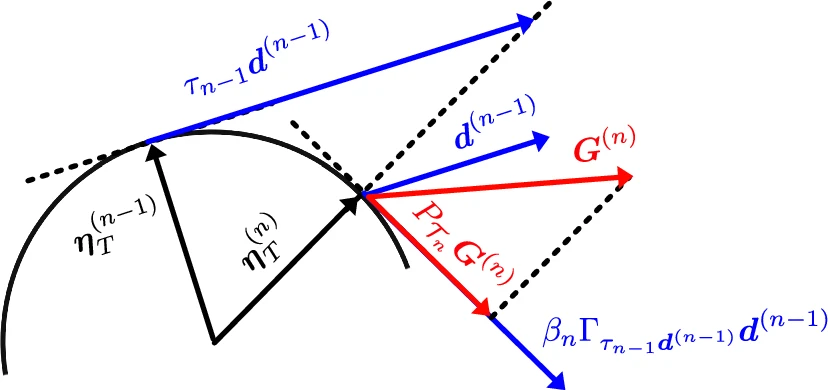
\includegraphics[width=.9\linewidth]{riemannian.png}
\caption{(Zhao et al. 2023, Fig. 1)}
\end{figure}
\Emp
}


\frame
{
\hspace*{-1.0cm}
\Bmp{12cm}
\raggedright

\begin{itemize}

\item<1->
Periodic algorithm restart $(\beta_n = 0)$
\begin{itemize}
\item<1->
\begin{equation*}
n = 20k, \quad k\in \ZZ^+
\end{equation*}

\item<2->
The search direction $\d^{(n)}$ is not an ascent direction
\begin{equation*}
\frac{\la \d^{(n)}, P_{\T_n}\bds G^{(n)} \ra_{G^\sigma}}{\|\d^{(n)}\|_{G^\sigma}\|P_{\T_n}\bds G^{(n)}\|_{G^\sigma}} < \epsilon, \quad 0<\epsilon \ll 1.
\end{equation*}
\end{itemize}


\item<4->
Iterations are stopped when the relative change of $\pat$ is below a specified tolerance
\begin{equation*}
0 \leq \frac{\pat(\benpa) - \pat(\bena)}{\pat(\bena)} < tol.
\end{equation*}

\end{itemize}
\Emp
}


\frame{
\centering

\LARGE
{Numerical Methods}
}


\frame
{
\hspace*{-1.0cm}
\Bmp{12cm}
\raggedright

\begin{itemize}

\item<1->
Discretized in space using a standard pseudospectral Fourier method 

\item<2->
Derivatives are evaluated in the Fourier
space

\item<3->
Nonlinear products are computed in the physical space on an uniform
grid with N points in each direction.

\item<4->
Explicit fourth-order Runge-Kutta

\item<5->
2/3 dealiasing

\end{itemize}
\Emp
}


\frame
{
\hspace*{-1.0cm}
\Bmp{12cm}
\raggedright

\begin{itemize}
\item<1->
Domain
\vspace{-0.25cm}
\begin{subequations}
\begin{align*}
\text{resolution}&: 128^3, 256^3, 512^3, 1024^3 \\
\alpha&: 1/1024, 2/1024, 4/1024, 8/1024, 16/1024 \\
\end{align*}
\end{subequations}
\vspace{-1.0cm}

\item<2->
Time
\vspace{-0.25cm}
\begin{subequations}
\begin{align*}
dt&: 2^{-5} \\
T&: 3, 5 \\
\end{align*}
\end{subequations}
\vspace{-1.0cm}

\item<3->
Gevrey class
\vspace{-0.25cm}
\begin{subequations}
\begin{align*}
\sigma&: \text{1E-5, 1E-4, 1E-3, 1E-2, 1E-1} \\
s&: 3
\end{align*}
\end{subequations}


\end{itemize}
\Emp
}

\section{Results}

\frame{
\centering

\LARGE
{Results}
}

\frame
{
\hspace*{-1.0cm}
\Bmp{12cm}
\raggedright

\begin{itemize}
\item<1->
Evolution of $\|\ua(\x,t)\|_{\hdo}^2$ over time for $\alpha=16/1024.$
\begin{figure}
\centering
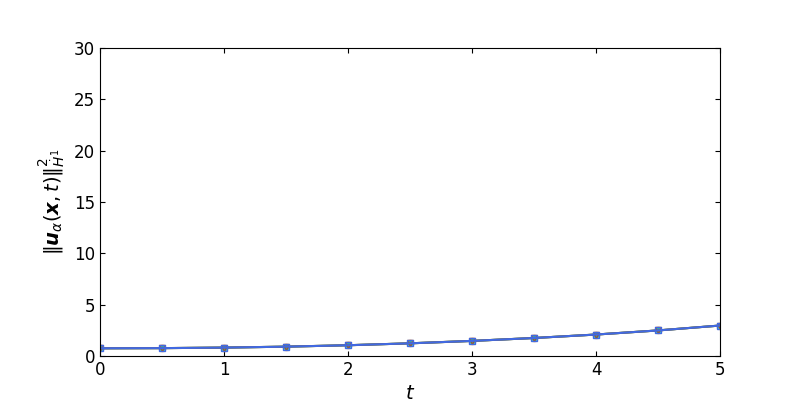
\includegraphics[width=.9\linewidth]{Figure_4_16.png}
\caption{Results for $\alpha=16/1024$. Results from runs performed at different resolutions are displayed together: $128^3$ (orange plus), $256^3$ (cyan star), $512^3$ (brown triangles), and $1024^3$ (blue squares).}
\end{figure}

\end{itemize}
\Emp
}

\frame
{
\hspace*{-1.0cm}
\Bmp{12cm}
\raggedright

\begin{itemize}
\item<1->
Evolution of $\|\ua(\x,t)\|_{\hdo}^2$ over time for $\alpha=8/1024.$
\begin{figure}
\centering
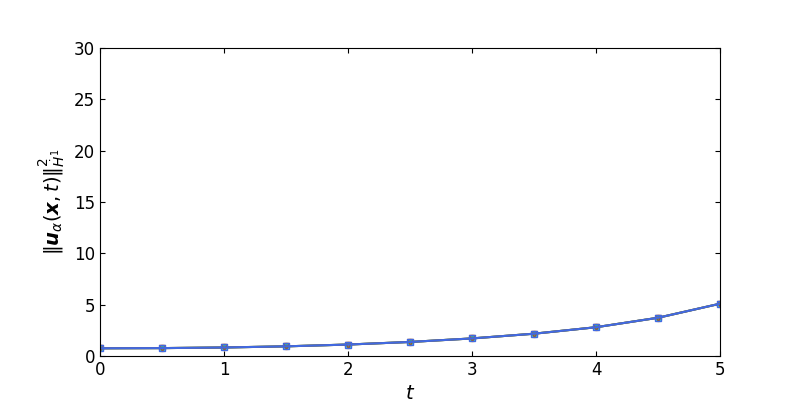
\includegraphics[width=.9\linewidth]{Figure_5_8.png}
\caption{Results for $\alpha=8/1024$. Results from runs performed at different resolutions are displayed together: $128^3$ (orange plus), $256^3$ (cyan star), $512^3$ (brown triangles), and $1024^3$ (blue squares).}
\end{figure}

\end{itemize}
\Emp
}

\frame
{
\hspace*{-1.0cm}
\Bmp{12cm}
\raggedright

\begin{itemize}
\item<1->
Evolution of $\|\ua(\x,t)\|_{\hdo}^2$ over time for $\alpha=4/1024.$
\begin{figure}
\centering
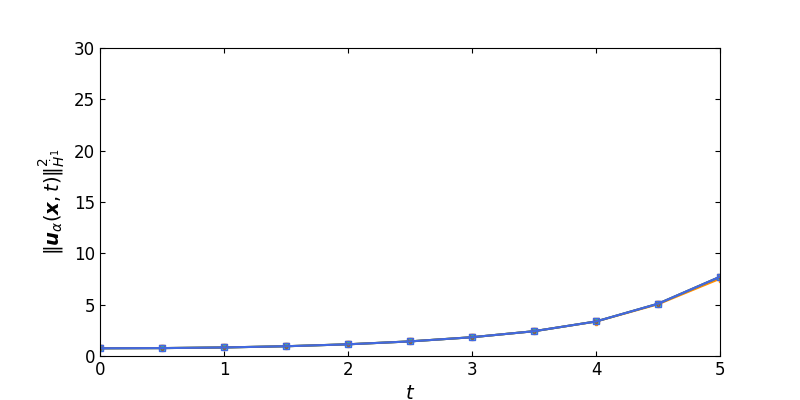
\includegraphics[width=.9\linewidth]{Figure_6_4.png}
\caption{Results for $\alpha=4/1024$. Results from runs performed at different resolutions are displayed together: $128^3$ (orange plus), $256^3$ (cyan star), $512^3$ (brown triangles), and $1024^3$ (blue squares).}
\end{figure}

\end{itemize}
\Emp
}

\frame
{
\hspace*{-1.0cm}
\Bmp{12cm}
\raggedright

\begin{itemize}
\item<1->
Evolution of $\|\ua(\x,t)\|_{\hdo}^2$ over time for $\alpha=2/1024.$
\begin{figure}
\centering
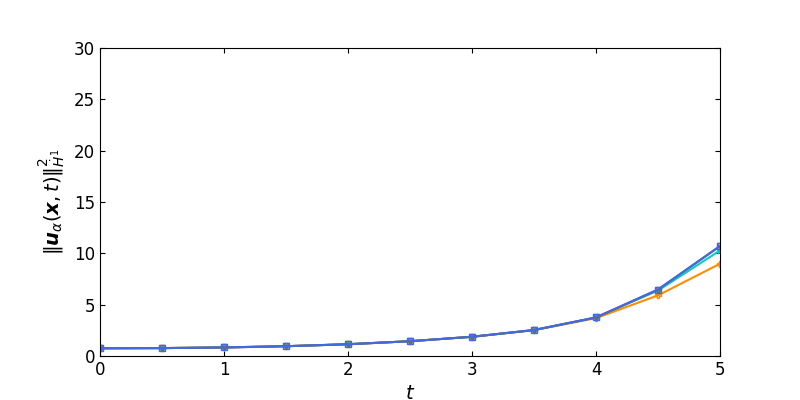
\includegraphics[width=.9\linewidth]{Figure_7_2.png}
\caption{Results for $\alpha=2/1024$. Results from runs performed at different resolutions are displayed together: $128^3$ (orange plus), $256^3$ (cyan star), $512^3$ (brown triangles), and $1024^3$ (blue squares).}
\end{figure}

\end{itemize}
\Emp
}

\frame
{
\hspace*{-1.0cm}
\Bmp{12cm}
\raggedright

\begin{itemize}
\item<1->
Evolution of $\|\ua(\x,t)\|_{\hdo}^2$ over time for $\alpha=1/1024.$
\begin{figure}
\centering
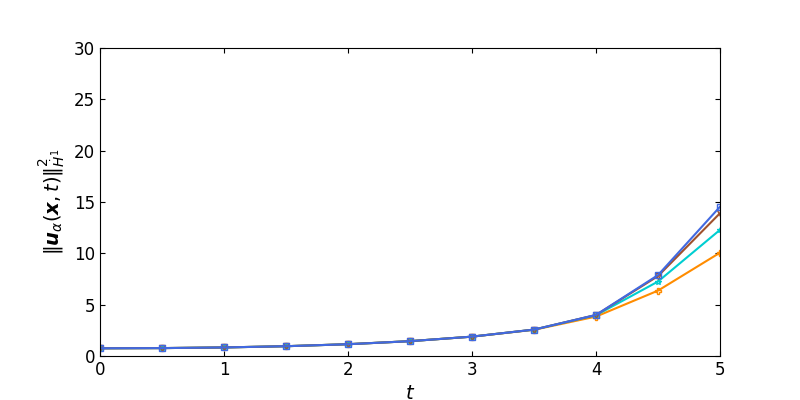
\includegraphics[width=.9\linewidth]{Figure_8_1.png}
\caption{Results for $\alpha=1/1024$. Results from runs performed at different resolutions are displayed together: $128^3$ (orange plus), $256^3$ (cyan star), $512^3$ (brown triangles), and $1024^3$ (blue squares).}
\end{figure}

\end{itemize}
\Emp
}

\frame
{
\hspace*{-1.0cm}
\Bmp{12cm}
\raggedright

\begin{itemize}
\item<1->
Evolution of $\|\u(\x,t)\|_{\hdo}^2$ over time for $\alpha=0.$
\begin{figure}
\centering
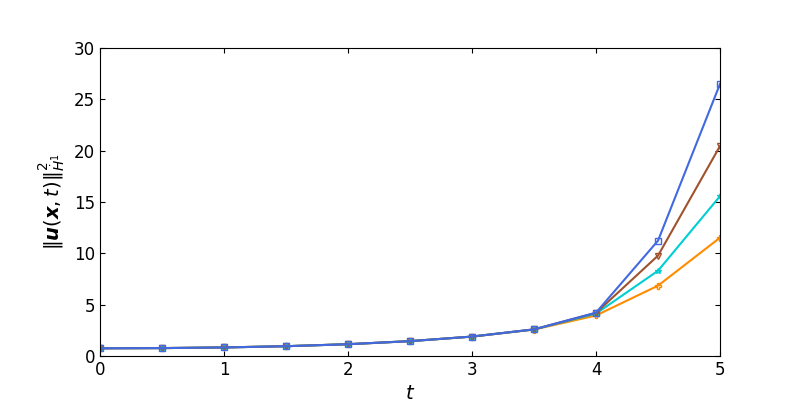
\includegraphics[width=.9\linewidth]{Figure_9_0.png}
\caption{Results for $\alpha=0$. Results from runs performed at different resolutions are displayed together: $128^3$ (orange plus), $256^3$ (cyan star), $512^3$ (brown triangles), and $1024^3$ (blue squares).}
\end{figure}

\end{itemize}
\Emp
}

\frame
{
\hspace*{-1.0cm}
\Bmp{12cm}
\raggedright

\begin{itemize}
\item<1->
Results of $\alpha^2\pat(\beza)$ as $\alpha\rightarrow 0$ for each resolution at $T=3,5$.
\begin{figure}
\centering
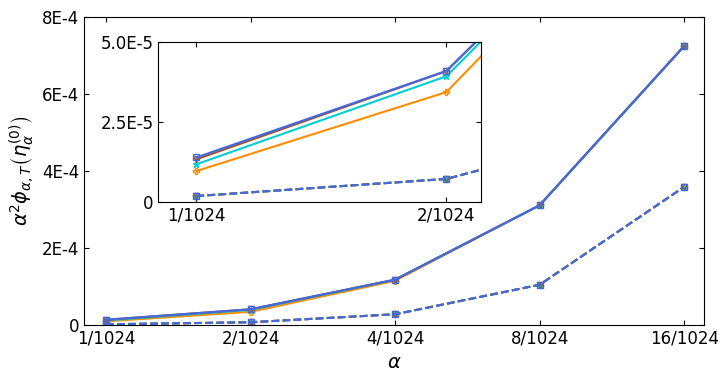
\includegraphics[width=.9\linewidth]{Figure_3.png}
\caption{Results for $T=3$ (dotted line) and for $T=5$ (solid line). Results from runs performed at different resolutions are displayed together: $128^3$ (orange plus), $256^3$ (cyan star), $512^3$ (brown triangles), and $1024^3$ (blue squares).}
\end{figure}

\end{itemize}
\Emp
}




\end{document}